\documentclass[a4paper]{article}

\usepackage[a4paper,  margin=0.5in]{geometry}
% \usepackage[left=2.5cm,top=3cm,right=2.5cm,bottom=3cm,bindingoffset=0.5cm]{geometry}

\usepackage{graphicx}
\usepackage{float}
\usepackage{hyperref}
\usepackage{multicol}


\usepackage[utf8]{inputenc}
\begin{document}

% \begin{titlepage}
\title{SNR classes project - birds species recognition using deep neural networks
- second stage report}

\author{Michał Sypetkowski, Marcin Lew}
\maketitle


\begin{multicols}{2}

\section{General information}
Git repository: 
\url{https://github.com/msypetkowski/SNR-proj.git}.
Previous stage report: 
\url{https://github.com/msypetkowski/SNR-proj/blob/master/doc/main.pdf}.

\section{Establishing Layers count}

First, we experiment with layers count.
    We trained 3 different models (they have respectively 11, 8 and 6 layers).
Detailed layers descriptions for each model are shown in tables respectively
\ref{table:layers11},
\ref{table:layers8} and
\ref{table:layers6}.
Rounded total trainable parameters count is respectively: 2.0M, 1.7M  and 1.5M.

Batch normalization with relu activation layers are used in all these models,
where the horizontal lines occur in the tables.

\begin{table}[H]
    \caption{ 11 layer convolutional NN architcture
    \label{table:layers11}
    }
\begin{center}
    \begin{tabular}{| l | l | l | l |}
    \hline
        Layer & kernel/window& strides & output shape\\
    \hline
        Conv1  & (5, 5)&        (1, 1)&     224x224x64  \\
    \hline
        MaxPool1 & (2, 2)&      (2, 2)&     112x112x64  \\
        Conv2  & (5, 5)&        (1, 1)&     112x112x64  \\
    \hline
        MaxPool2 & (2, 2)&      (2, 2)&     56x56x64    \\
        Conv3  & (5, 5)&        (1, 1)&     56x56x64    \\
    \hline
        MaxPool3 & (2, 2)&      (2, 2)&     28x28x64    \\
        Conv4  & (5, 5)&        (1, 1)&     28x28x64  \\
    \hline
        MaxPool4 & (2, 2)&      (2, 2)&     14x14x64  \\
        Conv5  & (5, 5)&        (1, 1)&     14x14x64  \\ % additional
    \hline
        MaxPool5 & (2, 2)&      (1, 1)&     14x14x64  \\
        Conv6  & (5, 5)&        (1, 1)&     14x14x64  \\
    \hline
        MaxPool6 & (2, 2)&      (2, 2)&     7x7x64  \\
        Conv7  & (5, 5)&        (1, 1)&     7x7x64  \\  % additional
    \hline
        MaxPool7 & (2, 2)&      (1, 1)&     7x7x64  \\
        Conv8  & (3, 3)&        (1, 1)&     7x7x128\\
    \hline
        MaxPool8 & (2, 2)&      (2, 2)&     4x4x128  \\
        Conv9  & (2, 2)&        (1, 1)&     4x4x128)\\
    \hline
        MaxPool9 & (2, 2)&      (1, 1)&     4x4x128  \\
        Conv10 & (2, 2)&        (1, 1)&     4x4x128)\\  % additional
    \hline
        MaxPool10 & (2, 2)&      (1, 1)&     4x4x128  \\
        Conv11 & (3, 2)&        (1, 1)&     4x4x128)\\  % 4x4
    \hline
        MaxPool11 & (2, 2)&      (1, 1)&     4x4x128  \\
        Flatten & - & - & 2048 \\
        Dense1 & - & - & 512 \\
    \hline
        Output & - & - & 50 \\
        Softmax & - & - & 50 \\
    \hline
    \end{tabular}
\end{center}
\end{table}

\begin{table}[H]
    \caption{ 8 layer convolutional NN architcture (layer names correspond to some layers names in 11 layer architecture \ref{table:layers11})
    \label{table:layers8}
    }
\begin{center}
    \begin{tabular}{| l | l | l | l |}
    \hline
        Layer & kernel/window& strides & output shape\\
    \hline
        Conv1  & (5, 5)&        (1, 1)&     224x224x64  \\
    \hline
        MaxPool1 & (2, 2)&      (2, 2)&     112x112x64  \\
        Conv2  & (5, 5)&        (1, 1)&     112x112x64  \\
    \hline
        MaxPool2 & (2, 2)&      (2, 2)&     56x56x64    \\
        Conv3  & (5, 5)&        (1, 1)&     56x56x64    \\
    \hline
        MaxPool3 & (2, 2)&      (2, 2)&     28x28x64    \\
        Conv4  & (5, 5)&        (1, 1)&     28x28x64  \\
    \hline
        MaxPool4 & (2, 2)&      (2, 2)&     14x14x64  \\
        Conv6  & (5, 5)&        (1, 1)&     14x14x64  \\
    \hline
        MaxPool6 & (2, 2)&      (2, 2)&     7x7x64  \\
        Conv8  & (3, 3)&        (1, 1)&     7x7x128\\
    \hline
        MaxPool8 & (2, 2)&      (2, 2)&     4x4x128  \\
        Conv9  & (2, 2)&        (1, 1)&     4x4x128)\\
    \hline
        MaxPool9 & (2, 2)&      (1, 1)&     4x4x128  \\
        Conv11 & (3, 2)&        (1, 1)&     4x4x128)\\  % 4x4
    \hline
        MaxPool11 & (2, 2)&      (1, 1)&     4x4x128  \\
        Flatten & - & - & 2048 \\
        Dense1 & - & - & 512 \\
    \hline
        Output & - & - & 50 \\
        Softmax & - & - & 50 \\
    \hline
    \end{tabular}
\end{center}
\end{table}



\begin{table}[H]
    \caption{ 6 layer convolutional NN architcture (layer names correspond to some layers names in 11 layer architecture \ref{table:layers11})
    \label{table:layers6}
    }
\begin{center}
    \begin{tabular}{| l | l | l | l |}
    \hline
        Layer & kernel/window& strides & output shape\\
    \hline
        Conv1  & (5, 5)&        (1, 1)&     224x224x64  \\
    \hline
        MaxPool1 & (2, 2)&      (2, 2)&     112x112x64  \\
        Conv2  & (5, 5)&        (1, 1)&     112x112x64  \\
    \hline
        MaxPool2 & (2, 2)&      (2, 2)&     56x56x64    \\
        Conv3  & (5, 5)&        (1, 1)&     56x56x64    \\
    \hline
        MaxPool3 & (4, 4)&      (4, 4)&     28x28x64    \\
        Conv6  & (5, 5)&        (1, 1)&     14x14x64  \\
    \hline
        MaxPool6 & (2, 2)&      (2, 2)&     7x7x64  \\
        Conv8  & (3, 3)&        (1, 1)&     7x7x128\\
    \hline
        MaxPool8 & (2, 2)&      (2, 2)&     4x4x128  \\
        Conv11 & (3, 2)&        (1, 1)&     4x4x128)\\  % 4x4
    \hline
        MaxPool11 & (2, 2)&      (1, 1)&     4x4x128  \\
        Flatten & - & - & 2048 \\
        Dense1 & - & - & 512 \\
    \hline
        Output & - & - & 50 \\
        Softmax & - & - & 50 \\
    \hline
    \end{tabular}
\end{center}
\end{table}

\subsection{Results}
We use Adam optimizer and coross entropy as loss function.
We train each model for 5K iterations with 128 element batches.
Accuracy curves are shown in figure \ref{fig:layersAcc}.

Training accuracy increases faster for models with fewer layers.
Smaller networks naturally learn faster, but they have fewer degrees of freedom
and may get worse results in the end.
11 Layes network architecture shown to be too complicated for
our dataset and training method.
Best accuracy was achieved by medium -- 8 layer network.
We use this architecture for further experiments.

\begin{figure}[H]
    \caption[]{Accuracy curves for models with different layers count}
    \centering
    \includegraphics[page=2,width=0.5\textwidth]{curvesLayers.png}
    \label{fig:layersAcc}
\end{figure}

\end{multicols}


\end{document}
